\documentclass[]{jarticle}          % 一段組
%\documentclass[twocolumn]{jarticle} % 二段組

\textwidth 180mm
\textheight 255mm
\oddsidemargin -12mm
\topmargin -15mm
\columnsep 10mm

%\vspace{0.5cm} % 一段組の場合はコメントアウトした方が体裁がよいx
%] % 一段組の場合はコメントアウトする

\usepackage{styles/labheadings}
\usepackage[dvipdfmx]{graphicx,color}
\usepackage{amsmath,amssymb}
\usepackage{url}
% 追加
\usepackage[hang,small,bf]{caption}
\usepackage[subrefformat=parens]{subcaption}
\usepackage{float}
\captionsetup{compatibility=false}

\input{numerical_definition.tex}
% report.texと同じディレクトリにnumerical_definition.texを入れておけば上の書き方でもいいはずです

\usepackage[
  dvipdfm,
  bookmarks=true,
  bookmarksnumbered=true,
  colorlinks=true]{hyperref}
\AtBeginDvi{\special{pdf:tounicode EUC-UCS2}}

\pagestyle{labheadings}
\headerleft{全方位画像を用いたシーンの3次元モデルの作成とその活用}   % ヘッダの左側のタイトル
\headerright{2025年4月23日}  % ヘッダの右側のタイトル

\begin{document}

%\twocolumn % 一段組の場合はコメントアウトする

\vspace*{2ex}
\begin{center}
 {\Large \bf テクスチャの修正と自己位置推定}\\ % タイトル
 \vspace*{5mm}
 {\large M2 田川幸汰}% 発表者名
\end{center}

%\vspace{0.5cm} % 一段組の場合はコメントアウトした方が体裁がよいx
%] % 一段組の場合はコメントアウトする

%新しく作成したコマンド
% \newcommand{\reffig}[1]{\hyperref[#1]{図\ref{#1}}}
% \newcommand{\refeq}[1]{\hyperref[#1]{式(\ref{#1})}}
% \newcommand{\reftab}[1]{\hyperref[#1]{表\ref{#1}}}
% \newcommand{\refsec}[1]{\hyperref[#1]{\ref{#1}章}}
% \newcommand{\refsubsec}[1]{\hyperref[#1]{\ref{#1}節}}

% 数式
%\begin{equation}
%  数式記述  
%  \label{ラベル名}
%\end{equation}

% 図
% \begin{figure}[!ht]
%   \begin{center}
%     \includegraphics[scale=0.5]{figures/画像ファイル名}
%     \caption{キャプション名}
%     \label{ラベル名}
%   \end{center}
% \end{figure}

% リスト
% \begin{enumerate or itemize}
%   \item 
% \end{enumerate or itemize}

\section{概要}
3次元モデルのテクスチャに変更を施し、再現精度を高めた。主な変更点は以下の2点である。
\begin{enumerate}
  \item 側面テクスチャと床面テクスチャを四角形形状のテクスチャに変更
  \item テクスチャを裏側から取得しないように修正
\end{enumerate}
  
\section{テクスチャ形状の変更}
三角形のテクスチャを使用する場合、テクスチャ割り当て時にずれが生じやすく、見た目がちぐはぐになって再現精度が低下する\ref{one}。
\begin{figure}[H]
  \begin{center}
    \begin{tabular}{c}
      \includegraphics[width=0.9\textwidth]{figures/3dmodel1.png}
    \end{tabular}
  \end{center}
  \caption{3次元モデル}
  \label{one}
\end{figure}
また、三角形で構成することで面の数が多くなり、それに伴い必要なテクスチャの枚数も増加してしまう。
さらに、側面と床面でテクスチャの形状が異なると、管理が煩雑になる可能性が高くなる。

これらの問題を解決するために、床面についてもテクスチャ形状を四角形に統一する。
これにより、再現精度の向上やテクスチャ枚数の削減、管理の簡素化が期待できる。

ただし、床面のテクスチャは側面と異なり、形状が一定ではない。
そのため、テクスチャの四隅の座標をもとにUV座標を算出し、射影変換に用いる必要がある。

\subsection{UV座標の導出}
UV座標とはテクスチャを3次元オブジェクトの表面に貼り付けるための座標系である。
同一平面上に存在する3頂点$\mathbf{p}_0,\mathbf{p}_1,\mathbf{p}_2$に対して、UV座標を構成するU軸は以下のように定義する。
\begin{equation}
  \mathbf{u} = \frac{\mathbf{p}_1 - \mathbf{p}_0}{|\mathbf{p}_1 - \mathbf{p}_0|} 
\end{equation}
また、V軸はU軸と3頂点で構成される平面の法線ベクトル$\nU$の外積で定義する。
\begin{gather}
  \mathbf{n} = \frac{(\mathbf{p}_1 - \mathbf{p}_0) \times (\mathbf{p}_2 - \mathbf{p}_0)}{|(\mathbf{p}_1 - \mathbf{p}_0) \times (\mathbf{p}_2 - \mathbf{p}_0)|} \\
  \mathbf{v} = \mathbf{u} \times \mathbf{n}
\end{gather}
$\mathbf{p}_0$をUV座標系の原点として、頂点$\mathbf{p}_i$をUV座標に投影する。
\begin{gather}
  \mathbf{d}_i = \mathbf{p}_i - \mathbf{p}_0 \\
  u_i = \mathbf{d}_i \cdot \mathbf{u} \\
  v_i = \mathbf{d}_i \cdot \mathbf{v} \\
\end{gather}
また、UV座標は$[0,1]$の範囲のため、以下のようにシフトとスケーリングの処理を行った。
\begin{gather}
  \mathbf{uv'}_i = [u_i, v_i] - \min_j([u_j, v_j])\\
  \mathbf{uv''}_i = \mathbf{uv'}_i \cdot \frac{1}{\max_j([u_j, v_j])}\\
\end{gather}
計算されたUV座標は、生成されたテクスチャのひずみをなくすために用いる。ひずみをなくすための射影変換行列を求めるために、
opencvのgetPerspectiveTransformメソッドを用いる。
また、射影変換行列を用いた画像変換にはopencvのwarpPerspectiveメソッドを用いる。

\subsection{生成されたテクスチャ}
生成された側面テクスチャ及び床面テクスチャを図\ref{two}に示す。
\begin{figure}[H]
  \begin{center}
    \begin{tabular}{cc}
      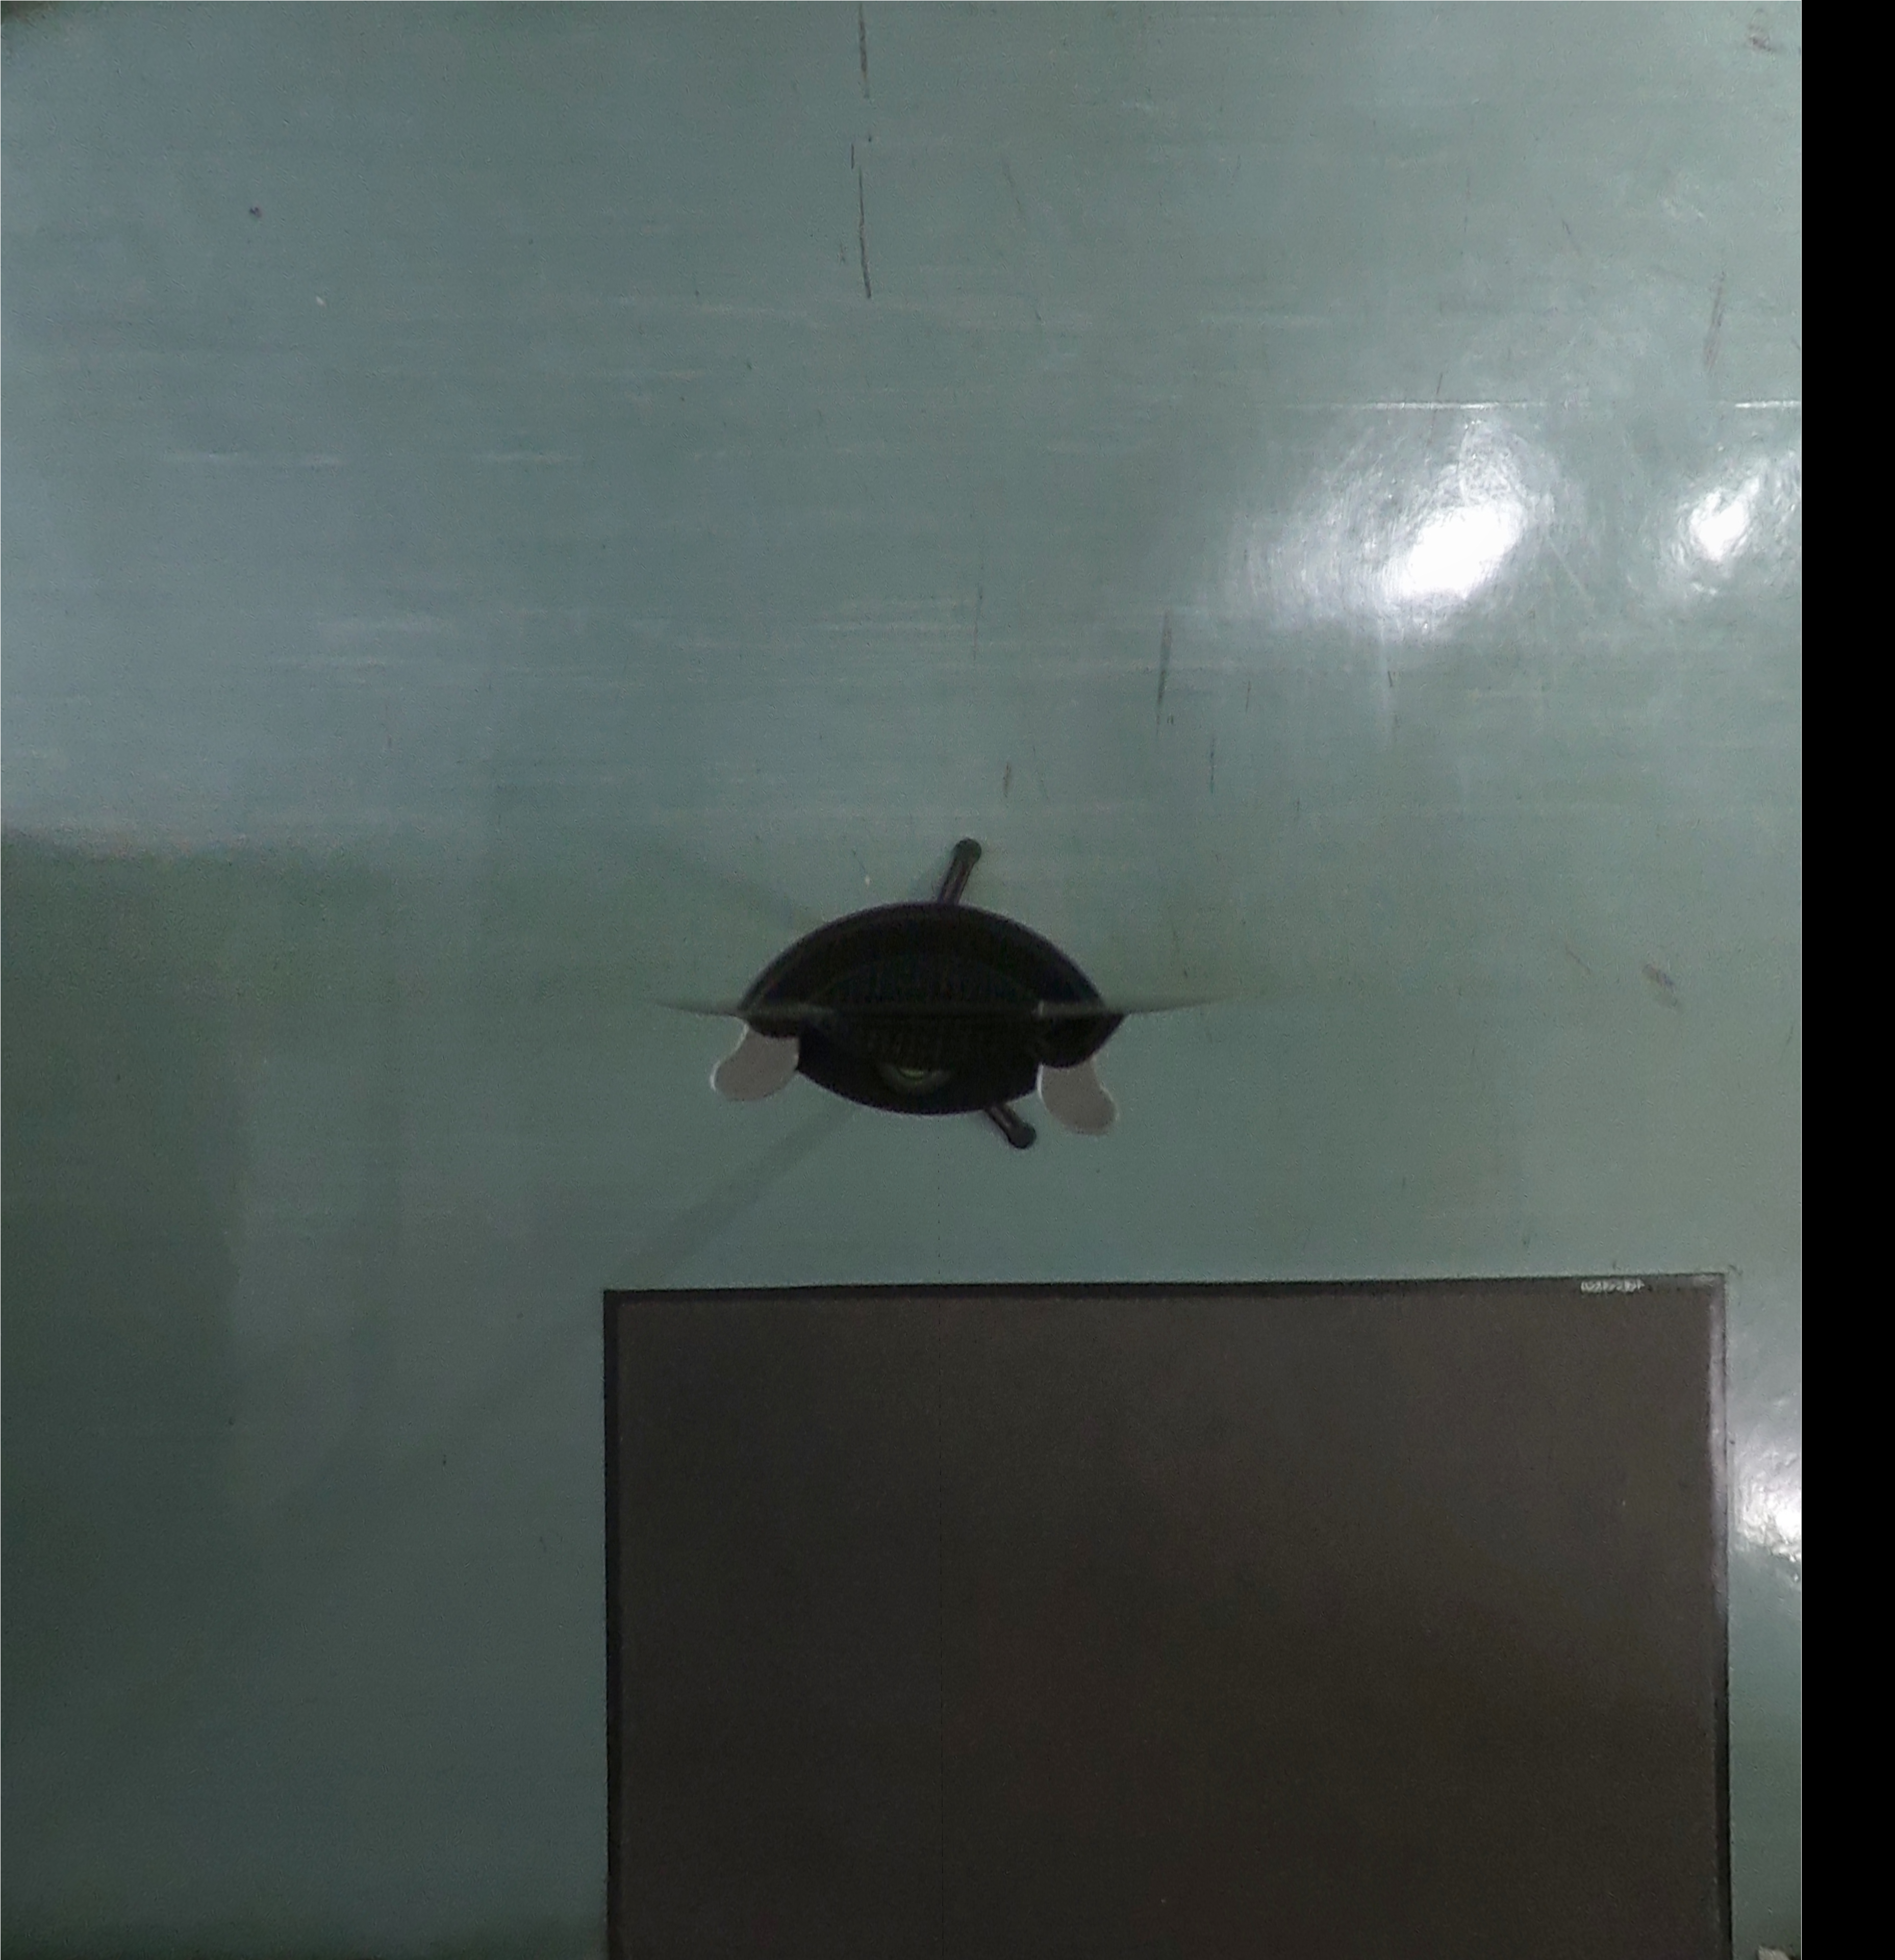
\includegraphics[width=0.4\textwidth]{figures/texture_0_0.png}&
      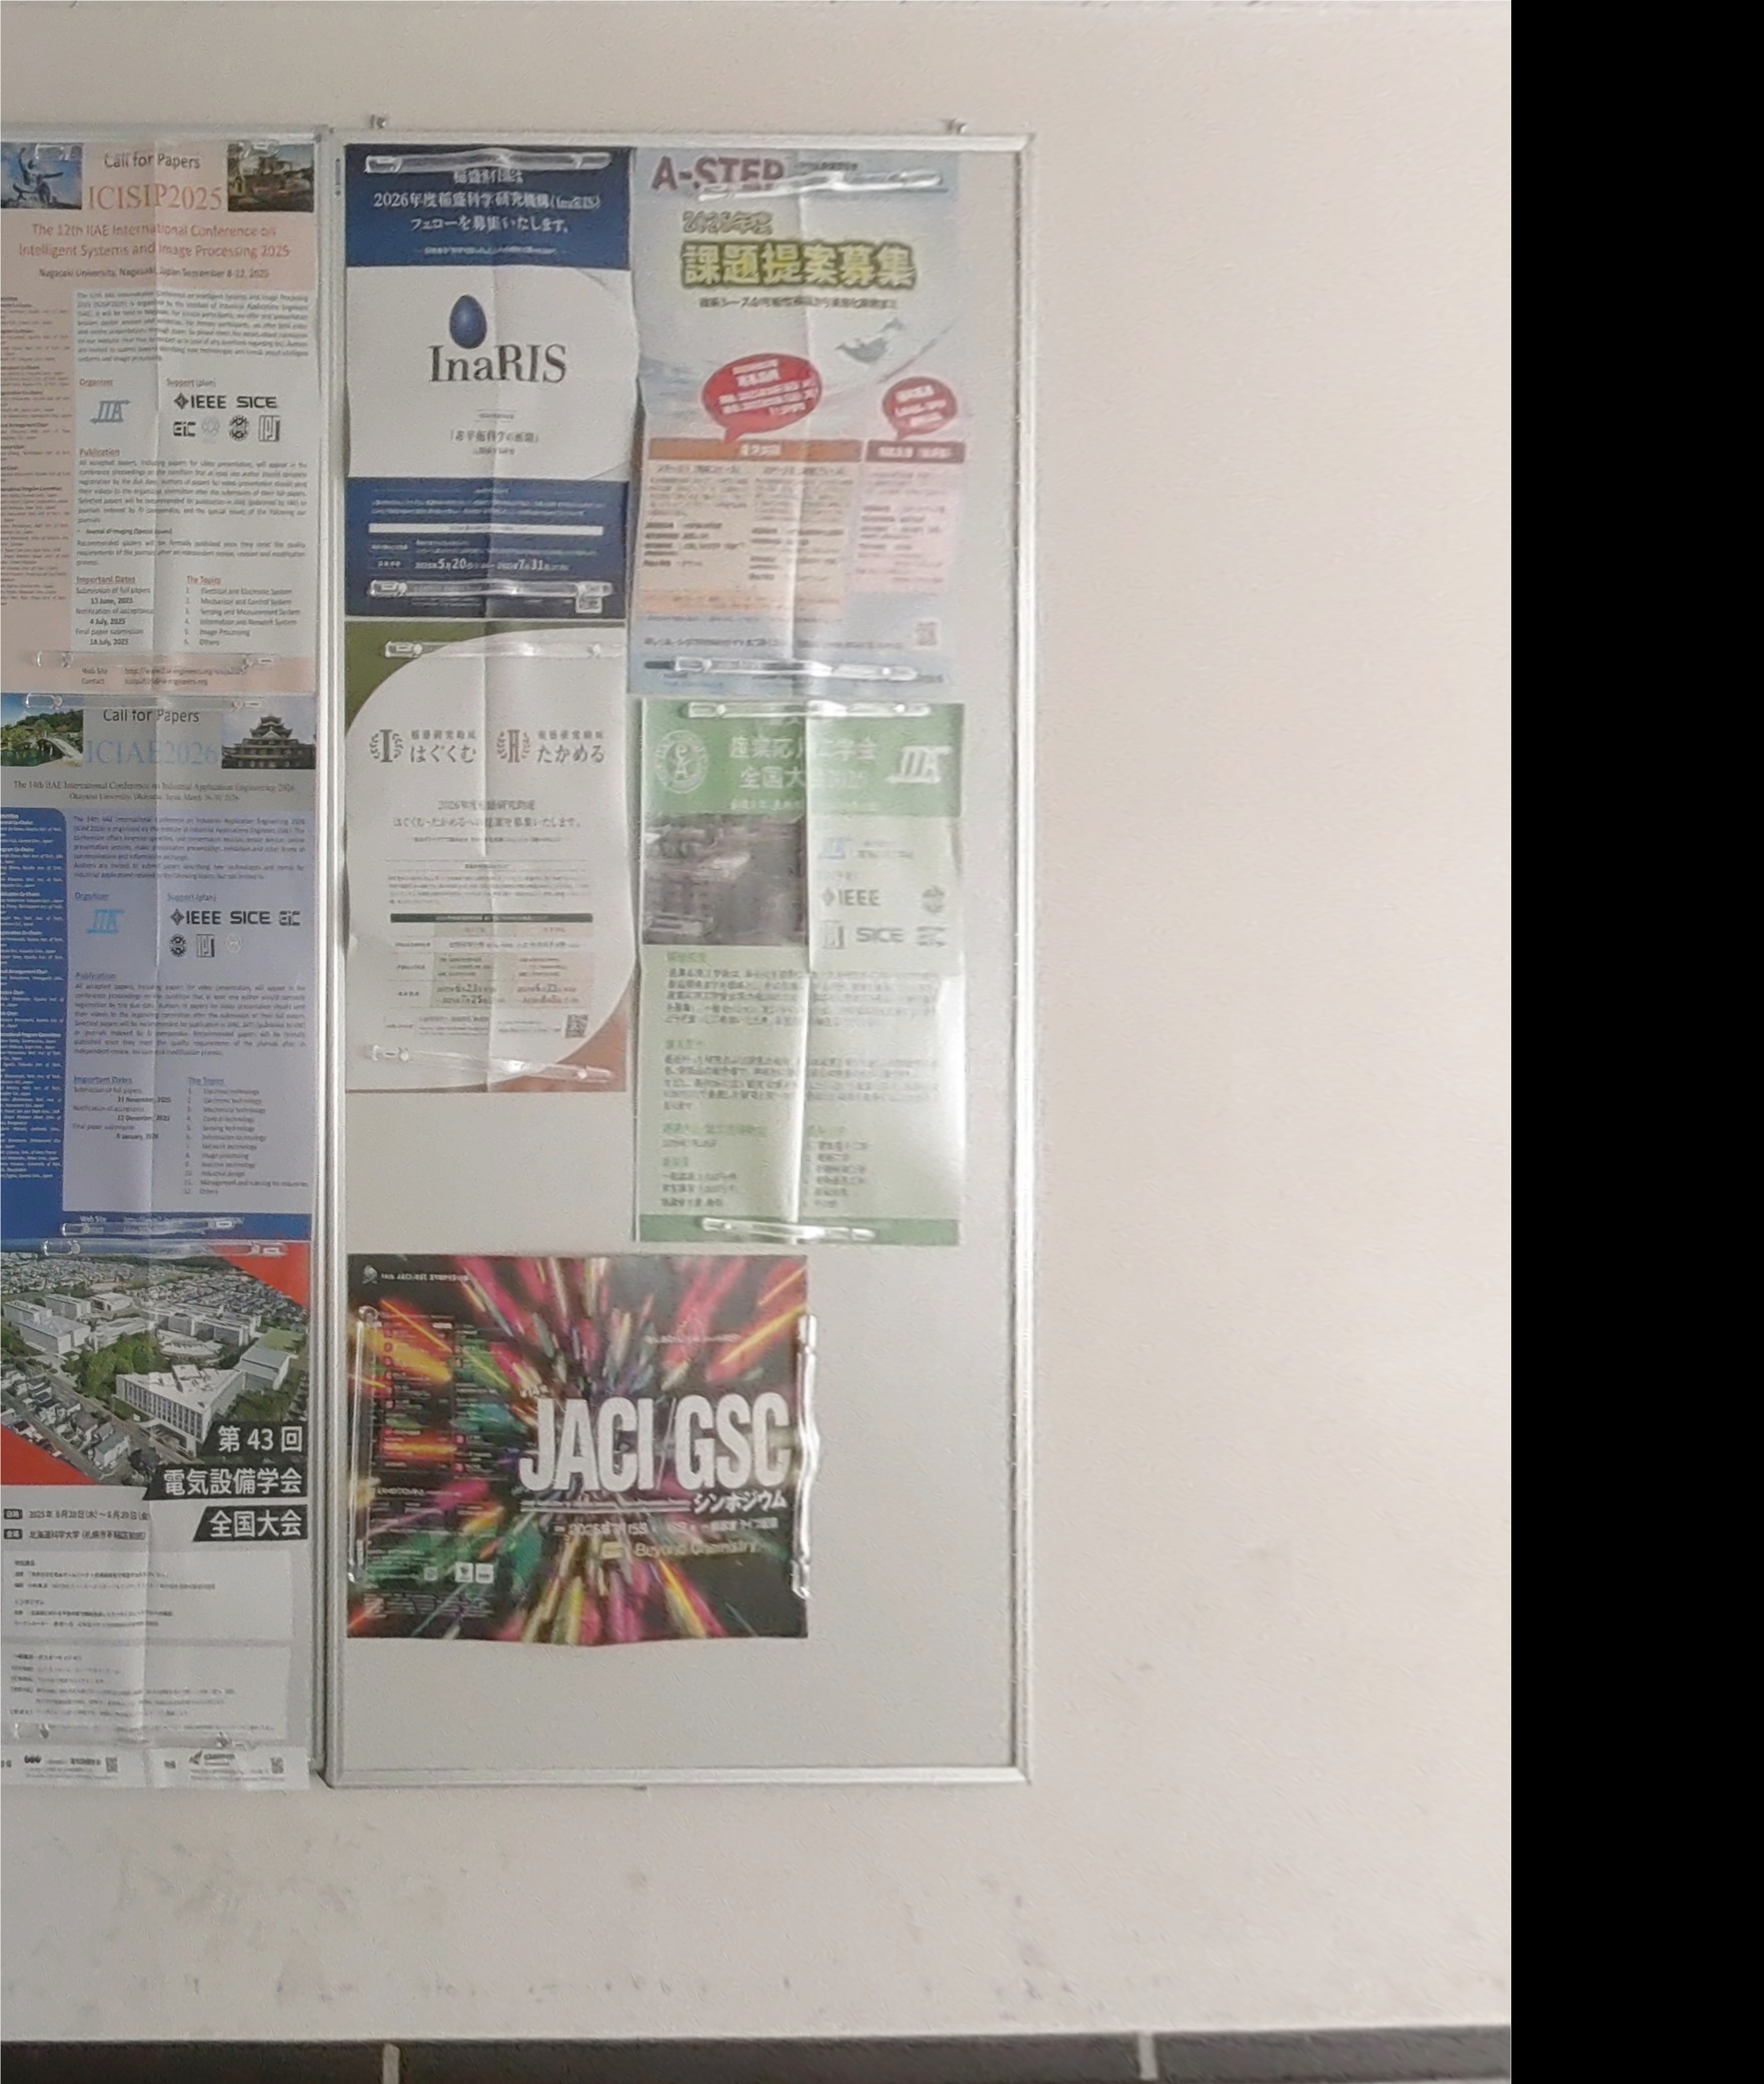
\includegraphics[width=0.4\textwidth]{figures/texture_2_30.png}\\
    \end{tabular}
  \end{center}
  \caption{テクスチャ画像}
  \label{two}
\end{figure}
床面、側面ともに正しく生成することができている。

\section{今後の計画}
今後の研究計画を以下に示す。
\begin{enumerate}
  \item 拡張した3次元モデルの側面部のテクスチャ割り当て
  \item 自己位置推定機能を応用した実用的なアプリケーションの開発
  \begin{itemize}
    \item 生成された3次元モデルと自己位置推定を組み合わせ、目的地までのルートを提示するナビゲーションシステムを構築
  \end{itemize}
\end{enumerate}
\end{document}
